\begin{figure}[htbp]
  \centering
  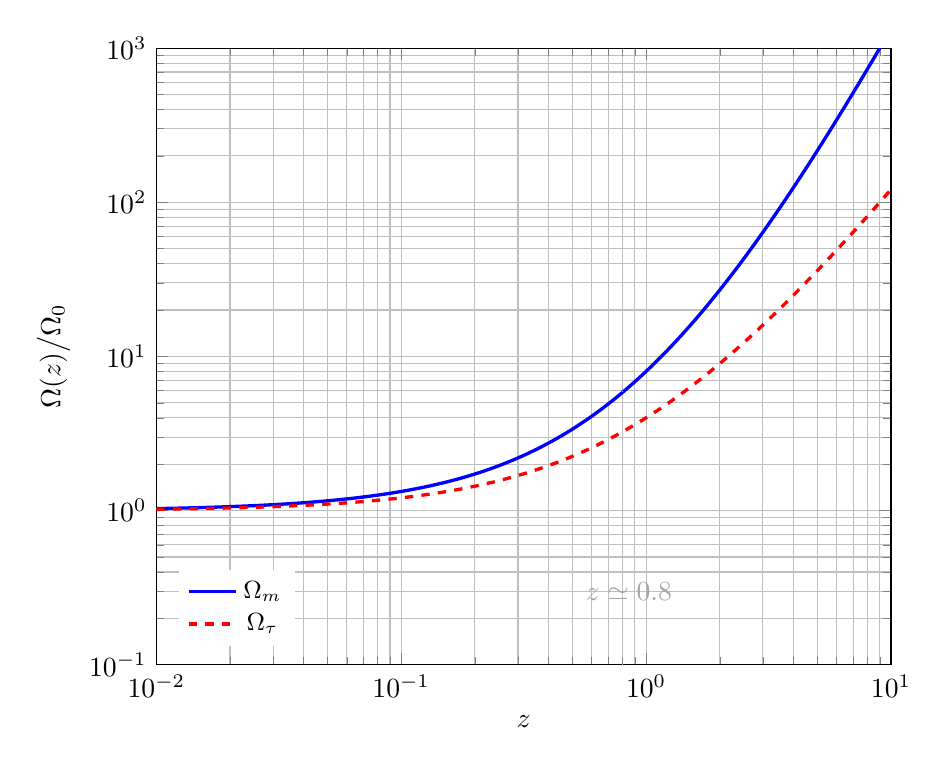
\begin{tikzpicture}
  \begin{axis}[
      width=0.9\textwidth,
      xlabel={$z$},
      ylabel={$\Omega(z)\big/\Omega_{0}$},
      xmode=log, ymode=log,
      xmin=0.01, xmax=10,
      ymin=0.1,  ymax=1000,
      grid=both,
      legend pos=south west,
      legend style={draw=none, font=\small}]
    % matter term  ∝ (1+z)^3
    \addplot[very thick,blue,domain=0.01:10,samples=180]{(1+x)^3};
    \addlegendentry{$\Omega_m$}
    % tau term  ∝ (1+z)^2
    \addplot[very thick,red,dashed,domain=0.01:10,samples=180]{(1+x)^2};
    \addlegendentry{$\Omega_\tau$}
    % vertical line at z ≈ 0.8
    \addplot[gray!60,dotted,domain=0.8:0.8] coordinates {(0.8,0.1) (0.8,1000)};
    \node[gray!70] at (axis cs:0.85,0.3) {$z\simeq0.8$};
  \end{axis}
  \end{tikzpicture}
  %-------------------------------------------------------------
  \caption{Evolution of the density parameters: $\Omega_m\propto(1+z)^3$ and $\Omega_\tau\propto(1+z)^2$. The cross-over at $z\!\approx\!0.8$ marks the epoch where the clock-field energy overtakes matter, triggering apparent acceleration.}
  \label{fig:MatterVsTau}
\end{figure}
